\capitulo{5}{Aspectos relevantes del desarrollo del proyecto}

En este apartado se van a mostrar los aspectos más importantes del
proyecto y los procesos que hemos seguido para el correcto funcionamiento de nuestra pagina con la debida conexión con la red Ethereum. Hablaremos de las herramientas utilizadas, pero la instalación de la mismas y la finalización de la página lo comentaremos en el apartado de los anexos.

El trabajo comenzó con la visita de la compañía HP a la universidad a exponer y realizar una charla sobre los TFG que se podían realizar con ellos durante el curso, para así empezar a realizar trabajos con una empresa real para un trabajo determinado.

\section{Comienzo del proyecto}

El trabajo comienza a partir de un proyecto que propone la empresa HP(Hewlett Packard) sobre aplicación de tecnología Blockchain a una cadena de distribución de productos. 

Una vez realizamos las primeras sesiones de para conocer al tutor de la empresa de HP: Pablo Tejedor García.

En la primera sesión decidimos los tiempos para realizar las diferentes tareas y ver la complejidad de cada una de ellas, todas las reuniones han sido realizadas vía llamada remota o presencialmente en la sede de León.

\section{Primeras sesiones}

En la primera sesión me recomendó la lectura del libro \textit{[Scrum y xp desde las trincheras]} el cual hemos comentando anteriormente, y la realización de programas básicos de prueba para la realización de la página en Visual Studio ya que le dije que habíamos usado esta herramienta durante la carrera y según algunos artículos era posible la conexión con la tecnología Blockchain, mediante la red web3 y la aplicación de la cual hablaremos mas adelante Metamask.


\section{Primer contacto con \textit{Ethereum}}

Una vez acabado y resumido el libro y realizados los primeros programas con Visual Studio, dimos el paso a la realización de nuestros primeros \textit{smart contract} 

En primer lugar, se decidió realizar un tutorial para tener unas tomas básicas en el ámbito de los \textit{smart contract}, ya que era la primera vez que utilizaríamos este tipo de lenguaje.

Este tutorial se realiza entero mediante Internet, se trata de una serie de capítulos los cuales te enseñan desde cero la creación de un contrato Solidity.

Hablaremos de ello en el apartado de trabajos relacionados en el punto siguiente.

\begin{figure}{l}
  \centering
  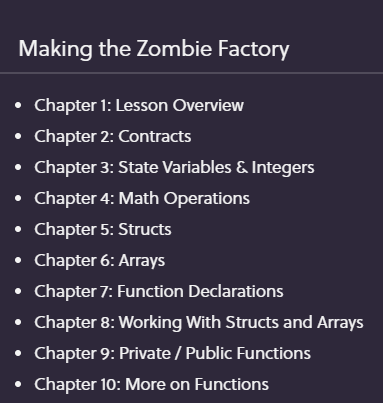
\includegraphics[width=0.5\textwidth]{zombie}
  \caption{Funciones: CryptoZombies}
\end{figure}  

Una vez concluido este proceso de iniciación en el mundo de Solidity, el siguiente paso era realizar pequeños contratos con cambio de dinero entre cuentas Ethereum, pero para empezar todas estas operaciones las realizamos mediante la opción localHost, esto lo conseguimos mediante dos formas.

\section{Realización de contratos en modo \textit{LocalHost}}

Para la realización de esto se empezó a usar una página de la cual no nos separemos a lo largo de nuestro proyecto, Remix.

Gracias a esté sitio web los smart contract que creemos se podrán probar directamente mediante la compilación.

Podremos seleccionar la versión con la que estamos trabajando y una vez compilado y sin errores, iremos a la pantalla de \textit{DEPLOY \& RUN TRANSACTIONS} una vez en esta página tendremos varias opciones 

En la opción \textit{Enviroment}, podremos elegir como se realizaran nuestros contratos:
\begin{itemize}
	\item JavaScript VM: esto nos crea 5 cuentas con una cantidad de 100 Ether en cada una, esto será una opción local para pequeñas pruebas, cuando cerreremos o ejecutemos otro programa la cuenta volverá a reiniciarse.
	\item Injected Web3: esta opción nos conectará directamente con Metamask, una vez que demos a \textit{deploy}, desplegar.
	\item Web3 Provider: en esta opción nos conectará con el servidor local de Ganache y nos dará acceso a las 10 cuentas que hay disponibles.
\end{itemize}
Con todas estas opciones nos creará un primer contrato, sin ningún valor mas que el gas de transacción.

Gracias al desplegable Account podremos seleccionar la cuenta en la que estemos, siempre y cuando no estemos en Injected Web3, ya que con esta opción siempre manejaremos la red desde Metamask.

Otro apartado es Gas limit se podrá indicar cuanto queremos y en caso de no poner un valor que sea inferior, nos mostrara error en este apartado. 

El ultimo parámetro que se puede modificar sera el valor que queremos indicar (Wei, Gwei o Ether), en caso de que nuestro contrato tenga una cantidad de divisa a enviar y no pongamos el valor, nos mostrará error de cantidad invalida.  

\begin{figure}[h]
  \centering
  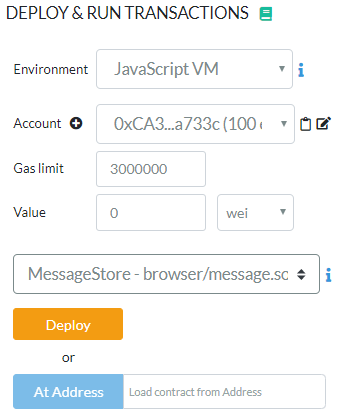
\includegraphics{remix-contract}
  \caption{Ejecutar contrato desde Remix}
\end{figure}  

\section{Creación de contratos desde Visual Studio}

Una vez fue entendida la herramienta con Remix, el siguiente paso fue la creación de una DApps, con las herramientas Visual Stuido, Tuffle, node.js y Ganache.

Primeramente tendríamos que instalar Node.js (\url{https://nodejs.org/en/}), una vez que fuera instalada instalaremos Truffle, y a continuación crearemos o ejecutaremos una carpeta  la cual contendrá los siguientes archivos:
\begin{itemize}
	\item contracts/: contiene los archivos Solidity que tendrán los contratos inteligentes.
	\item migratios/: sistema utilizado por Truffle para manejar las implementaciones de los smart contract. 
	\item test/: aquí realizaremos las pruebas Solidity y JavaScript para los smart contract
	\item truffle-config.js: archivo de configuración de Truffle.
\end{itemize}

Una vez tengamos la carpeta creada, escribiremos los smart contract, indicando la versión que deseemos usar de Solidity, cuando este finalizado nos encargaremos de compilar (truffle compile), y a continuación los migraremos\footnote{Migración: \textit{script} de implementación creado para alterar el estado de los contratos de su aplicación.} a nuestra cadena de bloques.

Anteriormente hablábamos de la herramienta Metamask, ahora para la conexión de desde Visual Studio a nuestro contrato, será necesario la instalación, la podremos descargar desde \url{https://metamask.io/}, es una extensión disponible para Chrome, Firefox, Opera, Brave, iOS y Android. También necesitaremos la aplicación Ganache, \url{https://www.trufflesuite.com/ganache}, este programa nos surtirá en modo local de diez cuentas, para poder trabajar con ellas, pero una vez que cerremos todo lo realizado de las transacciones se perderá.

El proceso de instalación de las herramientas anteriormente mencionadas lo comentaremos en el apartado de anexos.

Una vez tengamos Metamask tendremos que se crear o seleccionar la cuenta localhost:7545 será la encargada de conectar con Ganache, importando previamente las cuentas (con el código privado de la clave). 

Una vez tengamos todos creado, desde la terminal de Visual Studio (ctrl+ñ) tendremos que ejecutar npm run dev esto hará que el servidor se inicie y abra una pestaña en el navegador con el contenido de la dapp.

\begin{figure}[h]
  \centering
  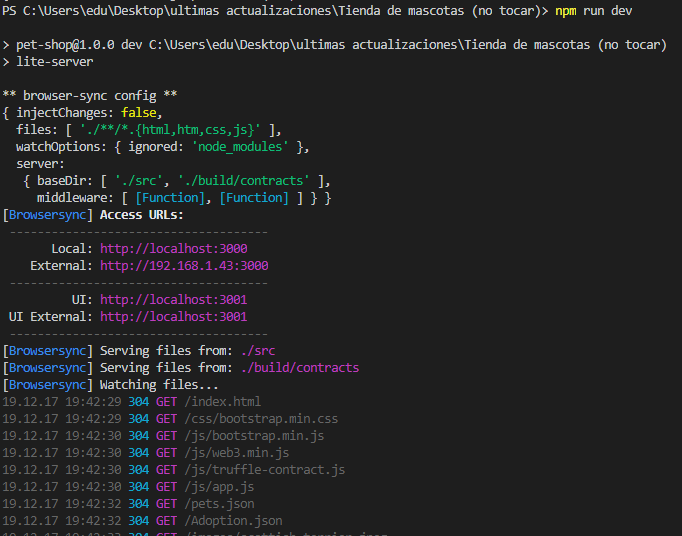
\includegraphics[width=1.00\textwidth]{npmrundev}
  \caption{Muestra de la ejecucción desde Visual Studio}
\end{figure}  

\section{Programas creados antes del programa final}

Antes de la creación final hemos realizado dos programas, ambos con conexión perfecta en ganache desde metamask, pero al intentar modificar las redes y tener que usar una red principal o privada, surgieron los mayores problemas, bien por problemas de divisa en Ether en las cuentas (debido a su dificultad de conseguir esta moneda en las redes, recordamos que en las redes locales que manejábamos anteriormente las divisas nunca se acaban ya que si reiniciamos la cuenta el dinero volvería al estado inicial de 100 Ether).

Los archivos que hemos creado son un servicio de compra de autobuses y una tienda de mascotas

\section{Empezando con redes privadas}

Al finalizar los contratos mediante la red con Ganache y comprobar que se realizaban correctamente el siguiente paso que nos propusimos fue la conexión de los smart contract con una red privada como son Ropsten, Rinkeby, Kovan.

Lo primero que hay que hacer es ingresar Ether en la cuenta, investigando por Internet descubrimos que había una página la cual permitía recaudar dinero pero solamente para la red Rinkeby.

El proceso para conseguir Ether consta de las siguientes partes:
\begin{enumerate}[1]
	\item Iremos a la página \url{https://plus.google.com/}, también se podrá realizar mediante la red de Twitter o Facebook y ahí tendremos que publicar el número de cuenta donde deseemos recibir el Ether.
	\item Una vez publicado copiaremos la url de nuestro post.
	\item Por ultimo en la pagina \url{https://www.rinkeby.io/#faucet} pegaremos la url y seleccionaremos el Ether que deseemos recibir, dependiendo la cantidad que escojamos no podremos realizar una nueva petición hasta que pasen los días  establecidos.
	\item Cuando se complete el proceso, podremos comprobar la cuenta y comprobar que el Ether aumento la cantidad seleccionada previamente.
\end{enumerate}

Ahora que ya tenemos dinero en nuestra red, podremos empezar a realizar smart contract desde Visual Stuido y conectar con las redes privadas mediante la aplicación que hace de intermediaria llamada Metamask. 
	 
\section{Problemas de conexión Web3}

En este punto en el cual ya disponíamos de dinero en nuestra red, intentamos la realización de poder ejecutar desde Visual Stuido a la red Ethereum, pero ya no en modo local como usábamos Ganache, si no realizarlo con Web3 y que realizara la conexión o con una red pública o privada.

Esto nos llevo mas de un quebradero de cabeza, ya que la conexión nos daba errores, por problemas de versiones de nuestro solidity y por asíncronos.

Nos planteamos el realizar una base de datos, la cual recogiera todos los datos y estos poder mostrarlos posteriormente, esto sin poder enseñarlos en la página de Etherscan.

Pero investigando y probando resulto que con la red privada Ropsten si que era posible realizar los contratos.

\section{Creación de la página}

Después de haber comprobado que nos permitía realizar los contratos de forma correcta y en la red privada, llego el momento de realizar la página web.

La cual hemos realizado con el programa XAMPP, es sistema de gestión de base de datos en MySQL y con Visual Stuido.

La pagina web hemos creado estas pantallas:
\begin{enumerate}[a]
	\item Inicio de sesión
	\item Nueva cuenta
	\item He olvidado la contraseña
	\item Mostrar opciones
	\item Añadir producto
	\item Consultar último producto
	\item Consultar productos existente
	\item Administrador de la cuenta
	\item Modificar datos del propio usuario
\end{enumerate}

Hablaremos más detenidamente del \textit{font-end} y \textit{back-end}, así como de la instalación de XAMPP en el apartado de los anexos.
